\documentclass[12pt]{article}
\usepackage{graphicx}
\usepackage{graphics}
\usepackage{refstyle}
\usepackage{amsmath}
\usepackage{caption}
\usepackage{float}
\usepackage{booktabs}
\usepackage{array}
\usepackage{physics}
\graphicspath{{/storage/self/primary/Download/latexnew/fig}}                                            
\graphicspath{{/storage/self/primary/Download/latexnew/table}}
\begin{document}
\title{\textbf{VECTOR}}
\date{}
\maketitle
\textbf{Question:}$\vec{P}$ and $\vec{Q}$ are any two points lying on the sides $DC$ and $AD$ respectively of a parallelogram $ABCD$.Show that, $ar(\triangle APB)=ar(\triangle BQC)$.


\textbf{Figure:}
\begin{figure}[H]
    \centering
    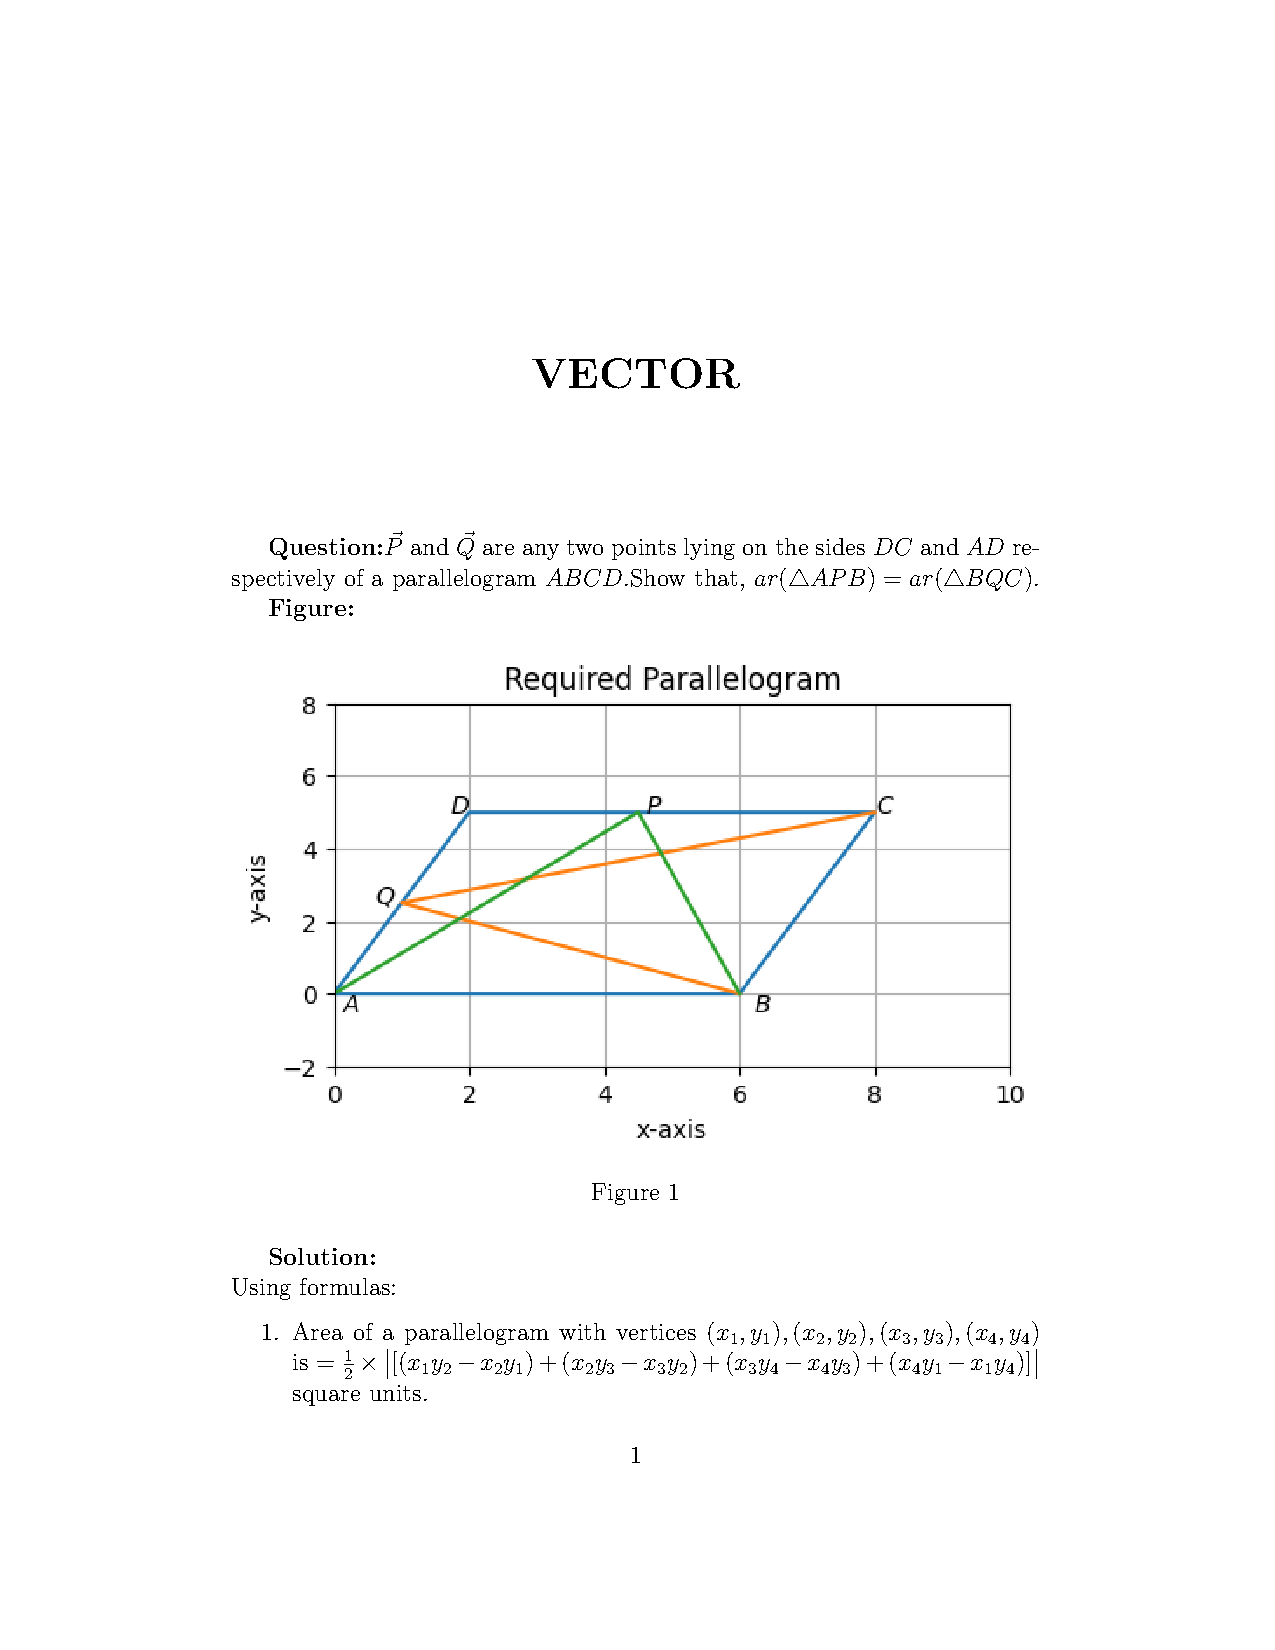
\includegraphics[width=\columnwidth]{fig/1.png}
    \caption{}
    \label{fig:fig:1}
\end{figure}


\textbf{Solution:}\\
Using formulas: \begin{enumerate}
\item Area of a parallelogram with  vertices $(x_1,y_1),(x_2,y_2),(x_3,y_3),(x_4,y_4)$ is =  $\frac{1}{2}\times \big |[(x_1y_2-x_2y_1)+(x_2y_3-x_3y_2)+(x_3y_4-x_4y_3)+(x_4y_1-x_1y_4)] \big|$ square units.
\item Area of a triangle with vertices $(x_1,y_1),(x_2,y_2),(x_3,y_3)$ is =  $\frac{1}{2}\times \big |x_1(y_2-y_3)+x_2(y_3-y_1)+x_3(y_1-y_2) \big|$ square units.

\item If a triangle and a parallelogram are on the same base and between the same parallels, then area of the triangle is equal to half the area of the parallelogram.

\end{enumerate}
From \figref{fig:1} ,
considering $\triangle BQC$ and parallelogram $ ABCD$, having \underline{same base $BC$} and, \underline{$AD$ is parallel to $BC$}.\\

\begin{equation}
\implies \triangle BQC = \frac{1}{2}\times ar ABCD.
 \label{eq:eq:1}
\end{equation}

Considering $\triangle APB$ and parallelogram $ABCD$ , having \underline{same base $AB$} and,\underline{$DC$ is parallel to $AB$}.

\begin{equation}
\implies \triangle APB = \frac{1}{2}\times ar ABCD.
 \label{eq:eq:2}
\end{equation}

By comparing \eqref{eq:1} and \eqref{eq:2} we obtain that,

\begin{equation}
    ar(\triangle APB) =  ar(\triangle BQC).
\end{equation}
\begin{center}
 Hence proved.

\end{center}

\textbf{Proof by the help of diagram :}(\figref{fig:1},\tabref{tab:1})
\begin{table}[H]
	\centering
	   \begin{tabular}{|c|c|c|}
    \hline
    \textbf{Input Parameters} &\textbf{Description} &\textbf{Value} \\
    \hline
     $\vec{O}$& Center(at origin)&$\vec{0}$\\
     \hline
 $r$ & Radius &1\\
 \hline
 $\theta$&-&$100\degree$\\
 \hline
 $\alpha$&-&$165.4\degree$\\
 \hline
 $\beta$&-&$5\degree$\\
 \hline
  \end{tabular}

	\caption{Table of input parameters}
	\label{tab:tab:1}
\end{table}


Let the points $\vec{P}$ and $\Vec{Q}$ divide $AD$ and $CD$ by $m_1:n_1$ and $m_2:n_2$ ratio respectively.

So,the coordinates of $\Vec{P}$ will be ($\frac{8m_1+2n_1}{m_1+n_1},\frac{5m_1+5n_1}{m_1+n_1}$) = ($\frac{8m_1+2n_1}{m_1+n_1}$,5) and, the coordinates of $\Vec{Q}$ will be ($\frac{2m_2}{m_2+n_2},\frac{5m_2}{m_2+n_2}$).\\
For the $\triangle APB$, the vertices of the triangle are

   $\Vec{A}=\begin{pmatrix}
       0\\0
   \end{pmatrix},
   \Vec{P}=\begin{pmatrix}
       \frac{8m_1+2n_1}{m_1+n_1}\\5
   \end{pmatrix},
   \Vec{B}=\begin{pmatrix}
       6\\0
   \end{pmatrix}$

   
$\implies \triangle APB = \frac{1}{2}\times \big |x_1(y_2-y_3)+x_2(y_3-y_1)+x_3(y_1-y_2) \big|$\\
$ = \frac{1}{2} \times \big |0(5-0)+\frac{8m_1+2n_1}{m_1+n_1}(0-0)+6(0-5)\big|\\
 = \frac{1}{2} \times\big |0+0-30\big|\\
 =\frac{1}{2} \times30\\
 =15 $ square units.


 For the $\triangle BQC$, the vertices of the triangle are
 
   $\Vec{B}=\begin{pmatrix}
       6\\0
   \end{pmatrix},
   \Vec{Q}=\begin{pmatrix}
       \frac{2m_2}{m_2+n_2}\\\frac{5m_2}{m_2+n_2}
   \end{pmatrix},
   \Vec{C}=\begin{pmatrix}
       8\\5
   \end{pmatrix}$

   
$\implies \triangle BQC = \frac{1}{2}\times \big |x_1(y_2-y_3)+x_2(y_3-y_1)+x_3(y_1-y_2) \big|$\\
$ = \frac{1}{2} \times \big |6(\frac{5m_2}{m_2+n_2}-5)+\frac{2m_2}{m_2+n_2}(5-0)+8(0-\frac{5m_2}{m_2+n_2})\big|\\
 = \frac{1}{2} \times\big |\frac{30m_2+10m_2-40m_2}{m_2+n_2}-30\big|\\
 =\frac{1}{2} \times30\\
 =15 $ square units.

 
  For parallelogram $ABCD$,the vertices are

   $\Vec{A}=\begin{pmatrix}
       0\\0
   \end{pmatrix},
 \Vec{B}=\begin{pmatrix}
       6\\0
   \end{pmatrix},
   \Vec{C}=\begin{pmatrix}
       8\\5
   \end{pmatrix},
   \Vec{D}=\begin{pmatrix}
       2\\5
   \end{pmatrix}$
   
$\implies ar ABCD = \frac{1}{2}\times \big |[(x_1y_2-x_2y_1)+(x_2y_3-x_3y_2)+(x_3y_4-x_4y_3)+(x_4y_1-x_1y_4)] \big|$\\
$ = \frac{1}{2} \times \big |[(0.0-6.0)+(6.5-8.0)+(8.5-2.5)+(2.0-0.5)] \big|
 = \frac{1}{2} \times\big |30+30\big|\\
 =\frac{1}{2} \times60\\
 =30 $ square units.

 
Or,By another method the area of the parallelogram $ABCD$ will be = $ a\times b \times \sin \theta$\\
 =$6\times\sqrt{29}\times \sin(\sin^{-1}{\frac{5}{\sqrt{29}}})$\\
=$6\times \sqrt{29} \times \frac{5}{\sqrt{29}}$\\
=30 square units.

Therefore,$ar ABCD = \frac{1}{2}\times ar \triangle APB = \frac{1}{2}\times ar \triangle BQC$(proved).


\end{document}
